\section{Day 1: Welcome, Transistors, and Electricity (Sept 2, 2025)}

We are trying to:
\begin{itemize}
    \item Understand computer software and hardware: Why is max int $2^{32} - 1$?
    \item How does Python evaluate \texttt{true} and \texttt{false}: Why are some values truthy? There's a hardware reason for that!\footnote{None, False, and generally numeric zero values and empty sequences/collections evaluate to false}
\end{itemize}

\noindent Why are we taking this course?
\begin{itemize}
    \item Understanding the machine, integrating software with hardware (e.g. sensors): such hardware skills can be rare these days
    \item Working with devices (Internet of Things)
    \item Satisfying prerequisites: stepping stones, a strong foundation
    \item You don't get a choice :D
\end{itemize}

\subsection{The Course at a Glance}
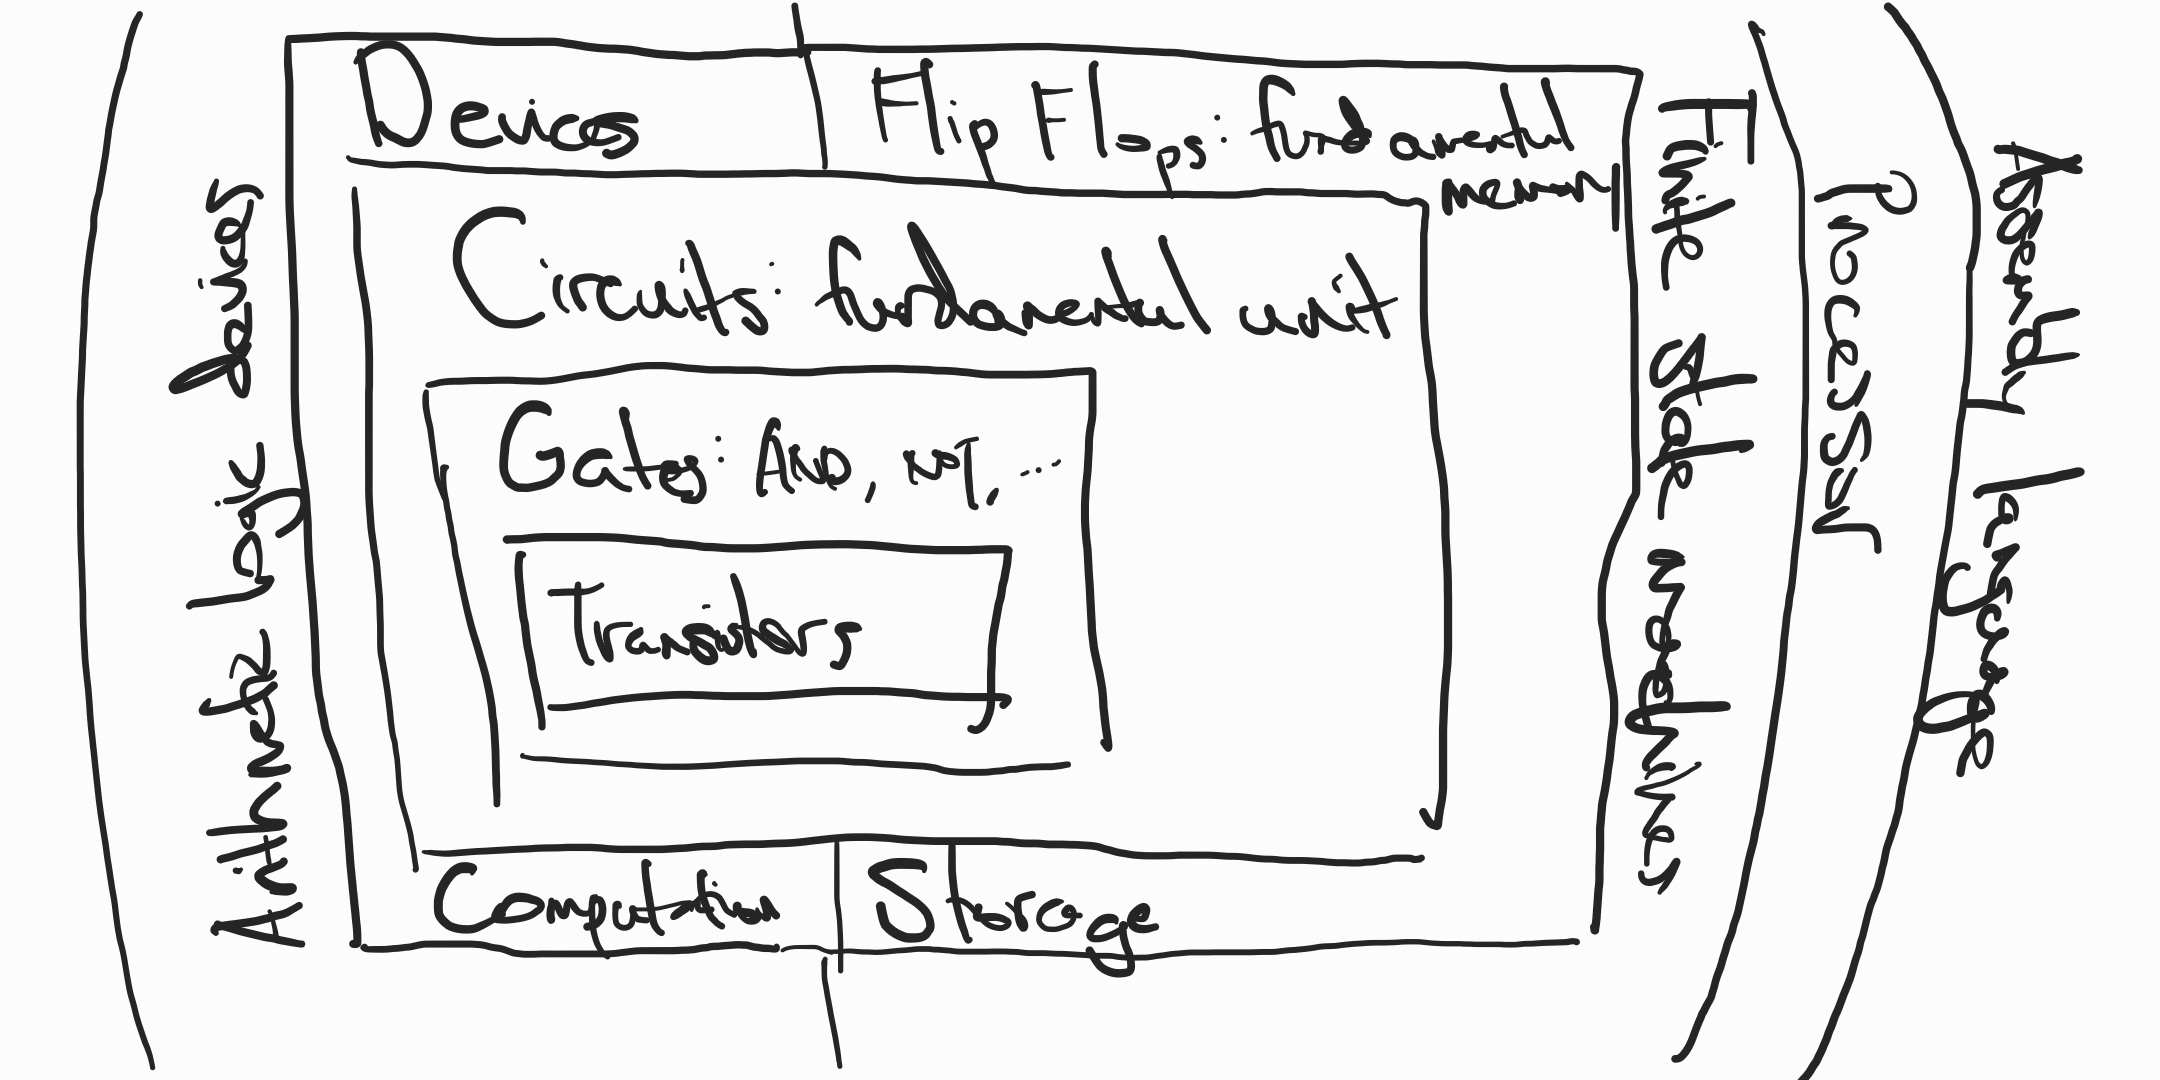
\includegraphics{csc258/figures/courseataglance.jpg}

\begin{remark}
    The tradeoff: we want a lot of transistors, because they speed up the processor, but they take up space, and we are reaching a physical limit as to how many we can stuff in a chip. Speeding up processors are not going to be as valuable, unless there is a significant breakthrough. Another way is to solve the problem using more \textit{efficient} circuits, CS Theory enthusiasts rejoice! We could also restrict circuits from being general purpose to more specialized designs that excel at a particular task.\footnote{an example can be GPUs and matrix multiplication}. All in all, there's a lot of active research, and utility for these thingamajigs.
\end{remark}

Logic gates are the hardware equivalent of propositional operators previously encountered. Common ones include: AND, OR, NOT, XOR. We will learn about the mysterious buffer gate, which has the following behavior: $0 \to 0$, $1 \to 1$, in later weeks. To implement logic gates, we will need \textit{transistors}, and we will later properly motivate why we need them. Logic gates can then be used to implement higher level behavior, like addition!

Unlike other CS courses, this course is about creating devices and machines, rather than programs and algorithms.

\subsection{Course Goals}

\begin{itemize}
\item Be able to create and design circuits, implement Finite State Machines
\item Understand microprocessor architecture
\item Understand assembly language
\item Learn about how lower-level languages and even hardware achieve higher-level behavior
\end{itemize}


\subsection{Administrative Details}
\begin{itemize}
\item 2 hours of lecture on Tuesday, with 1 hour of tutorial inbetween \\
Half of this tutorial is explaining what the lab is, and the other is a TA going over review material
\item 3 hour labs are more involved, note that you will be able to do most of the work at home. There are 7 total, 4\% each, starting on week 2. 
    \begin{itemize}
    \item Pre-lab: exercises submitted on Quercus \textbf{before} the lab
    \item Demo: performed for TAs, there may be follow up questions
    \end{itemize}
    You \textbf{must} show up to the lab you're enrolled in, they are assigned according to your last name
\item There is an Assembly Language Project worth 15\%:
    \begin{itemize}
    \item Create an interactive game in MIPS assembly
    \item 5 milestones worth 3\% each
    \item Milestone demos take place in the lab rooms. Think about finishing early because labs may get pretty busy towards the end of the year
    \end{itemize}
\item Midterm worth 19\% tentatively scheduled for Thurs Oct 16, 6pm-8pm
\item Final worth 38\%, need a 40\% to pass the course, with 3 hours time limit
\end{itemize}

\subsection{Transistors}

Transistors form the basic building blocks of all computer hardware, used for amplification, switching, and digital logic design. They made vacuum tubes obsolete, and made computing practical, since vacuum tubes keep breaking.

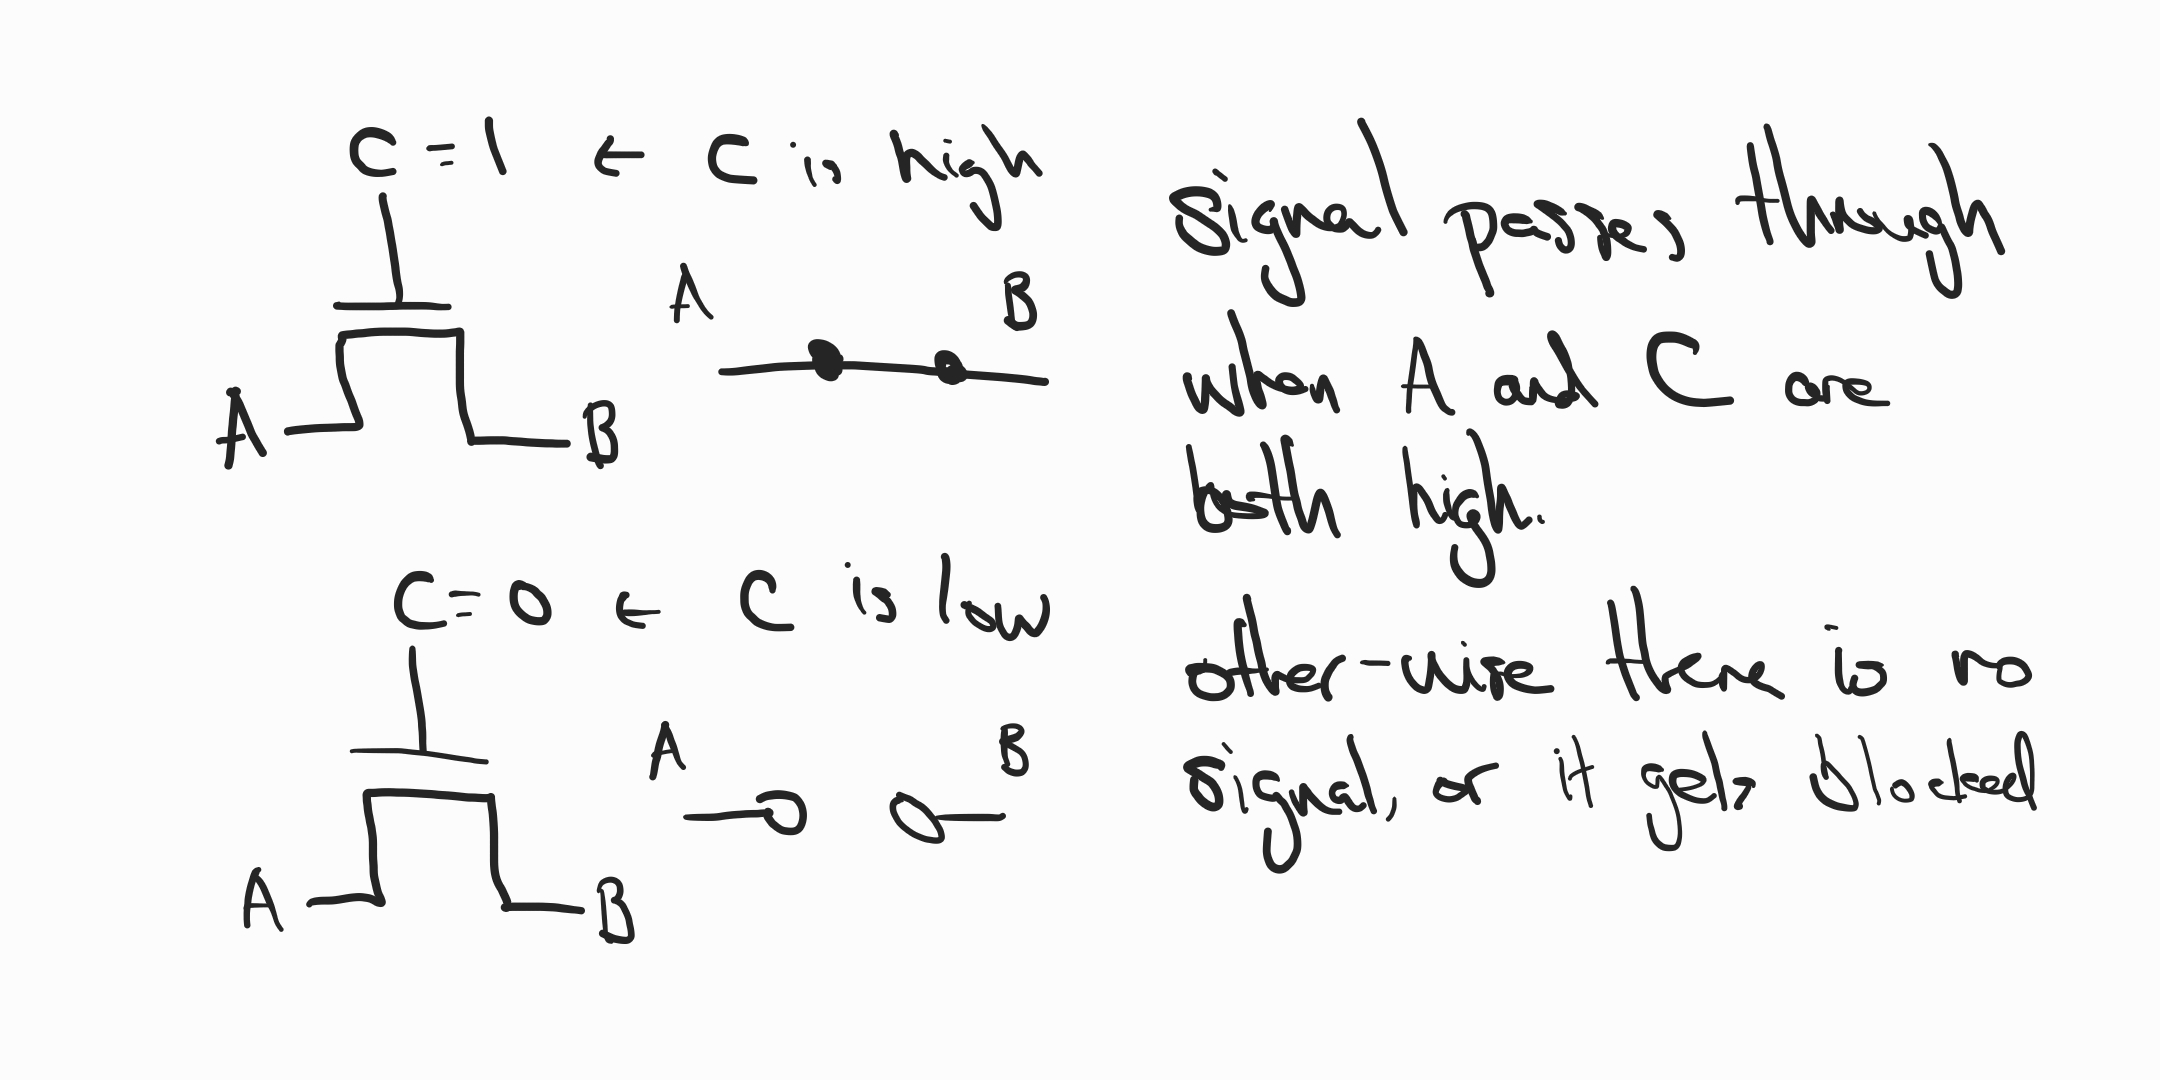
\includegraphics{csc258/figures/transistor.jpg}

When the transistor is on, then the value at point $B$ is determined by that of point $A$, in fact they are equal. Otherwise, the value at point $B$ cannot be determined from the values of point $A$.

To represent 2 different states, we need connect our wire to a battery (for high), and to ground (for low). Otherwise we may pick up some noise in a wire not connected to ground, and interpret it as high which is undesirable.

\begin{remark}
    Logic gates are made from transistors, based on pn-junctions, which are made from semiconductwhat's your name againwhat's your name againors which conduct electricity. (We don't need to know what pn-junctions nor semiconductors are)
\end{remark}

\subsection{Electricity}
\begin{definition}[High: Course Specific]
    5 Volts-ish
\end{definition}
\begin{definition}[Low: Course Specific]
    0 Volts-ish, or could be -5?
\end{definition}

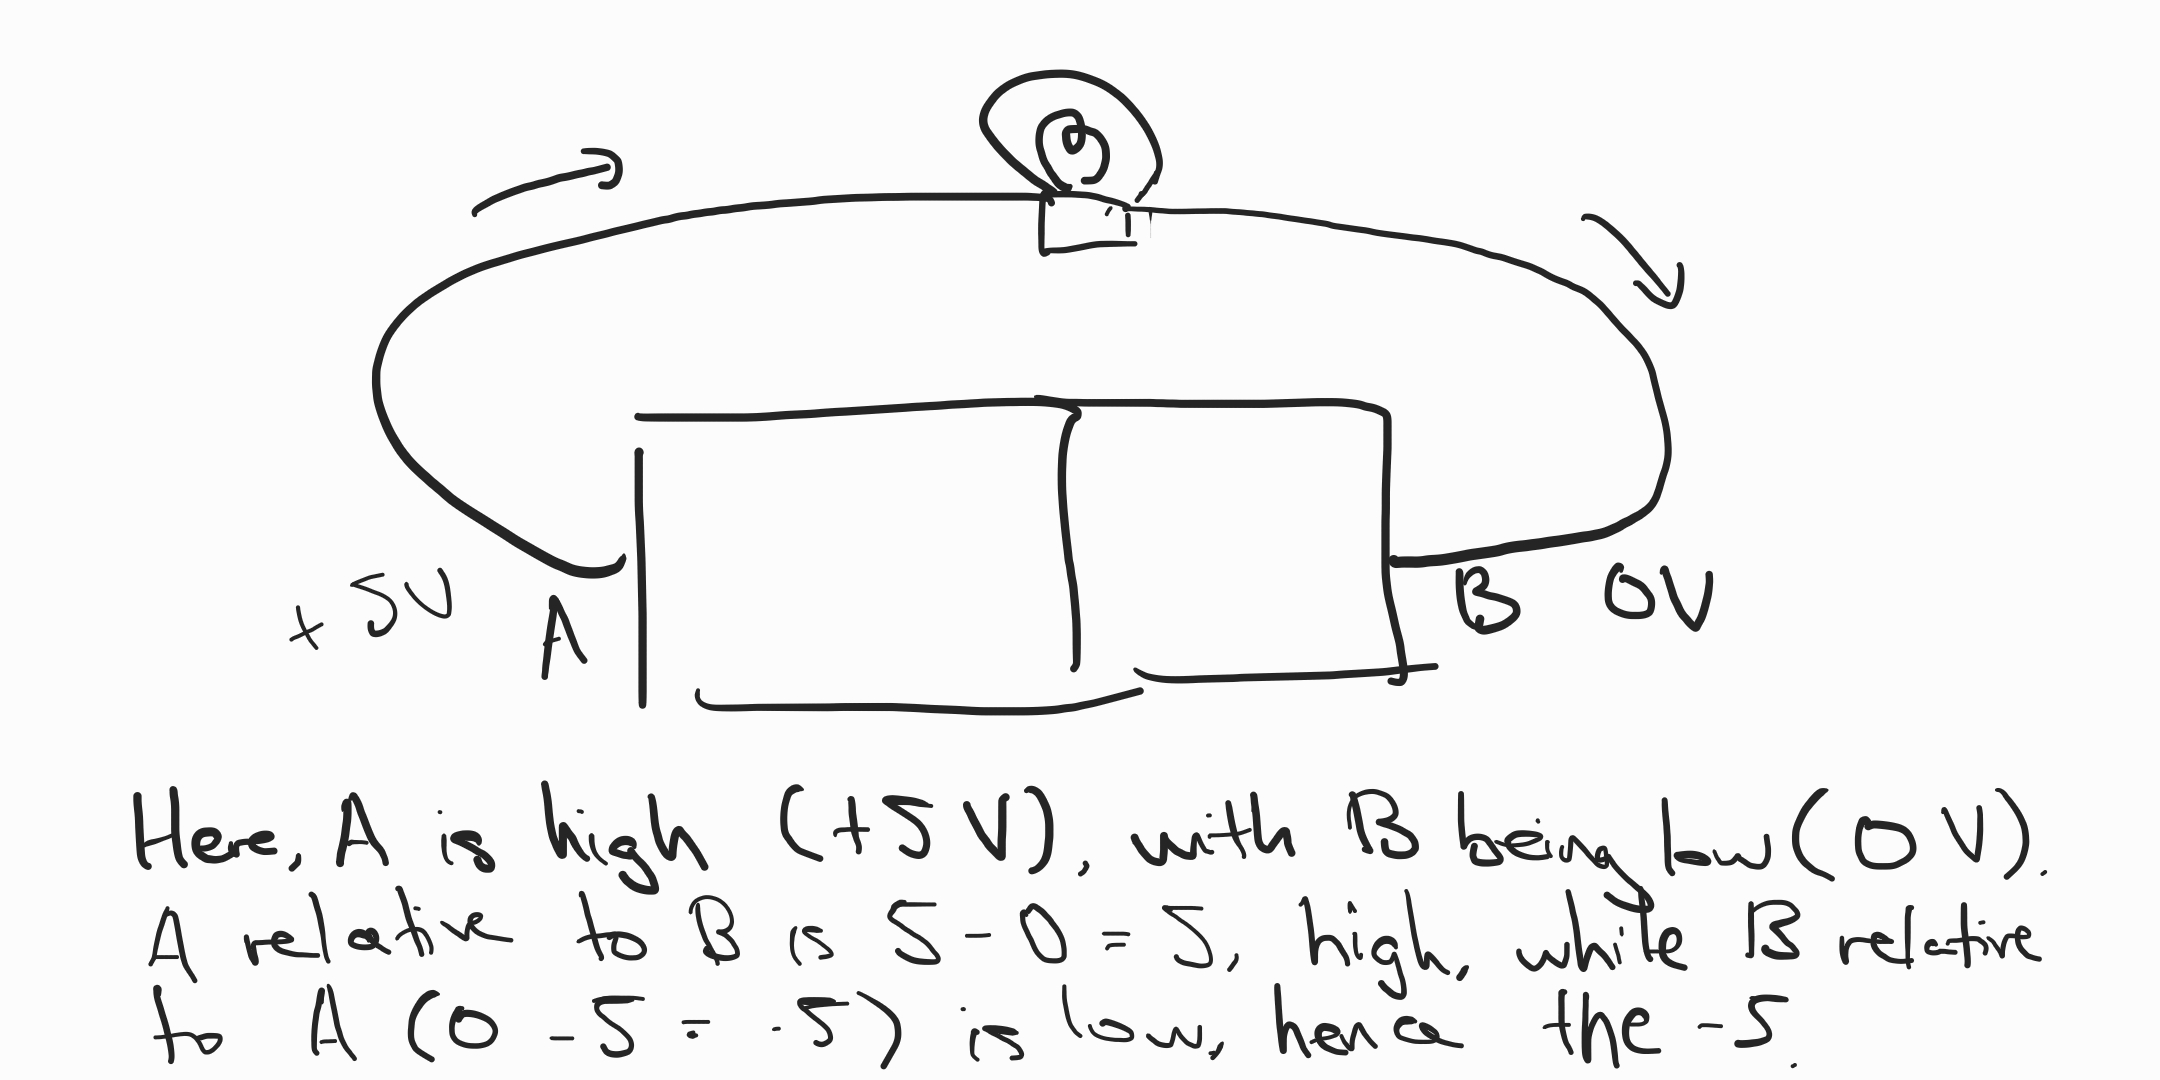
\includegraphics{csc258/figures/neg5explanation.jpg}

TODO: The reason -5 appears sometimes is because when you're measuring a low and compare it to a high, it will be -5, except when you measure 2 highs it'll show up as a low? Won't you always want to measure relative to ground or something idk.

\begin{definition}[Electricity]
    The flow of charged particles (usually electrons) through a material. 
\end{definition}
Charged particles can do \textit{work}, and originate from atoms. Electrons flow from regions of high electrical potential (many electrons) to regions of low electrical potential (few electrons). This potential\footnote{the reason this is called a potential because it hasn't actually happened yet - prof} is called \textbf{voltage}, and the rate of electron flow is called the \textbf{current}.

This means that voltage is almost always measured relative to something else. Current is influenced by voltage, as follows.

\begin{example}[Water Tower Analogy]
    \textbf{Voltage} is like the elevation of the water above the ground. \textbf{Current} is the rate at which the water flows. The more potential energy, the easier it is to unleash
\end{example}

\begin{definition}[Resistance]
    Denoted $R$, it is the relationship between voltage $V$ (measured in volts) and current $I$ (measured in amps).
\end{definition}
\[
R := \frac{V}{I}\footnote{also we say that resistance doesn't change a lot because ``the material isn't changing'' - prof}
\]

Electrical resistance indicates how well a material allows electricity to flow through it. \textbf{Insulators} have high resistance, do not conduct electricity well, with \textbf{conductors} having low resistance and conducting electricity well.

\begin{remark}
    Even though current is caused by electrons flowing, the convention is to measure current as the \textbf{movement of positive charges}, despite them not actually moving. Electrons moving from $A$ to $B$ make $A$ less negative and $B$ more negative. But (rather incorrectly) people conclude that positive charges are moving from $B$ to $A$, meaning $A$ is getting less positive and $B$ is getting more positive.
\end{remark}

Static electricity demonstrates this imbalance, which is caused by materials `stealing' electrons from each other. When an imbalanced object comes in contact or close enough with a balanced one (because electrons tend to not move through the air), extra electrons transfer over and there exists a \textit{current}, since electrons are flowing!

Sources of electricity include:
\begin{itemize}
\item Batteries have a concentration of particles stored, which will run out eventually
\item Outlets, which are constantly being supplied to avoid downtime
\end{itemize}

Current always flows toward the zero voltage point of a circuit, which is called \textbf{ground}, and takes the path of \textit{least resistance}. Each circuit has an \textit{source} (where the electrons come from) of electrical particles, some \textit{path} between this source and the \textit{ground} (destination), and some \textit{resistance} along this path that dissipates these electrons.

\begin{definition}[Semiconductor]
Exist somewhere inbetween conductors and insulators, which is a desirable property for transistors.
\end{definition}
